\chapter{Anforderungen und Konzept}
\section{Zielgruppenanalyse}
Die Zielgruppe der Web App sind Studierende technischer und medienorientierter Studiengänge, die einen hohen Bedarf an Selbstorganisation haben. Viele verwenden mehrere Tools wie Papierkalendar, Notizapps, Moodle oder Google Kalender. Die Web App soll eine zentrale und strukturierte Plattform zur Verfügung stellen.\newline \newline
Digital unterstützte Selbstorganisation durch Studierende wird zunehmend international adressiert. \textcite{obexer} zeigen, dass die Rolle sogenannter Learning Designers - als Brücke zwischen Technologie und didaktischem Einsatz - nicht nur Lehrende unterstützt, sondern auch Studierende in ihrem Lernprozess stärkt. Sie betonen, dass ohne gezielte Support-Strukturen digitale Tools oft fragmentiert und ineffizeint genutzt werden. 
\section{Funktionale Anforderungen}
Die Progressive Web App soll die folgenden zentralen Funktionen bereitstellen:

\begin{itemize}
  \item \textbf{Vorlesungsverwaltung:} Nutzer:innen sollen Vorlesungen hinzufügen, bearbeiten und löschen können.
  \item \textbf{Kalenderintegration:} Prüfungstermine, Abgabefristen und Veranstaltungen sollen im Kalender sichtbar und verwaltbar sein.
  \item \textbf{Notizmodul:} Studierende sollen in der Lage sein, Notizen zu Vorlesungen zu speichern, zu verschlagworten und gezielt zu durchsuchen.
  \item \textbf{Offline-Funktionalität:} Die Anwendung soll auch ohne Internetzugang nutzbar bleiben (PWA-Standard).
  \item \textbf{Synchronisation:} Daten sollen geräteübergreifend synchronisiert werden.
  \item \textbf{Gebrauchstaugliche Oberfläche:} Die Web App soll eine intuitive, barrierearme Oberfläche bieten.
\end{itemize}
\section{User Stories}
Als Student:in möchte ich meine Vorlesungen eintragen, um meinen Stundenplan digital zu organisieren.\\
Als Student:in möchte ich Notizen zu Vorlesungen speichern, um diese später leicht und schnell zufinden.\\
Als Student:in ohne Internetverbindung möchte ich meine Notizen offline einsehen können, damit ich auch unterwegs lernen kann.\\
Als Student:in möchte ich Prüfungstermine in einem Kalender verwalten, um keine Fristen zu verpassen.

\section{Grobkonzept und Mock-ups}
Die Abblindung \ref{fig:homepage} zeigt die Startseite der Web App, die eine Übersicht über alle Vorlesungen und anstehenden Termine bietet. Die Navigation ermöglicht den Zugriff auf den Stundenplan, Notizen und den Kalender.
\begin{figure}[H]
  \centering
  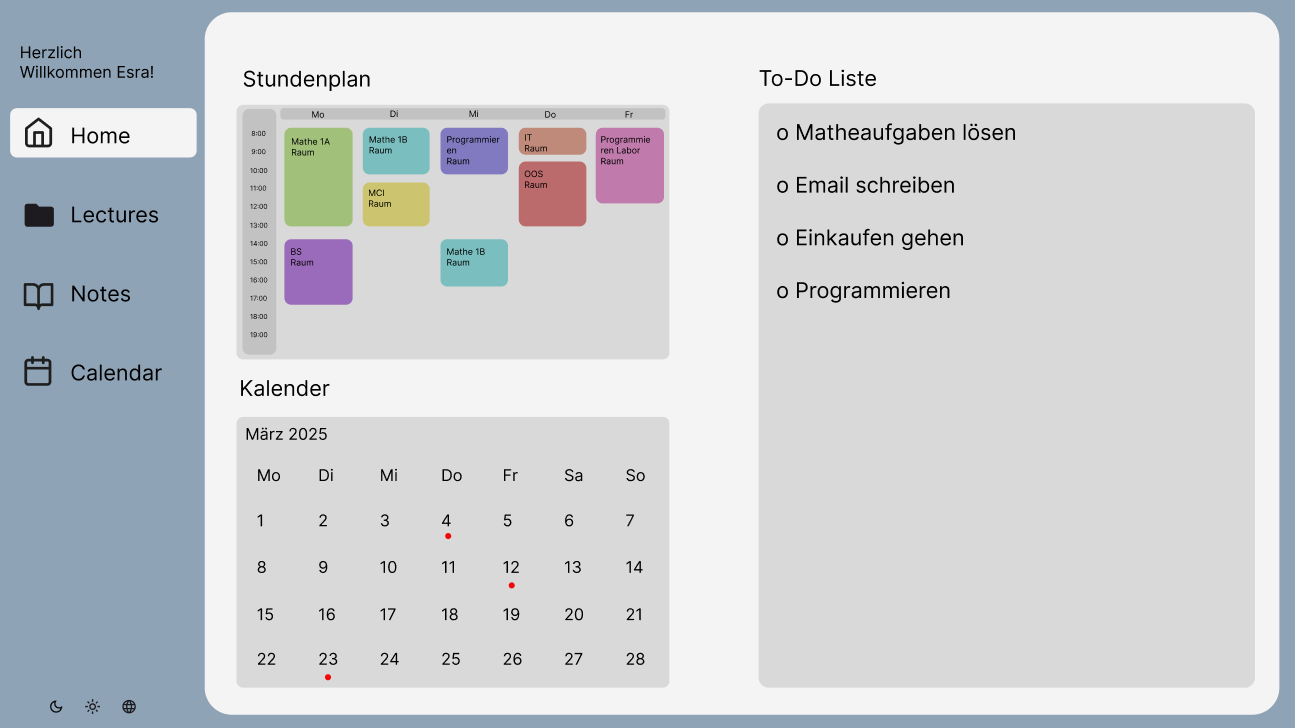
\includegraphics[width=1\textwidth]{./images/homepage.png}
  \caption{Startseite}
  \label{fig:homepage}
\end{figure}
In Abbildung \ref{fig:lectures} ist die Seite für die Verwaltung vom Stundenplan dargestellt. Hier können Nutzer:innen Vorlesungen hinzufügen, bearbeiten und löschen.
\begin{figure}[H]
  \centering
  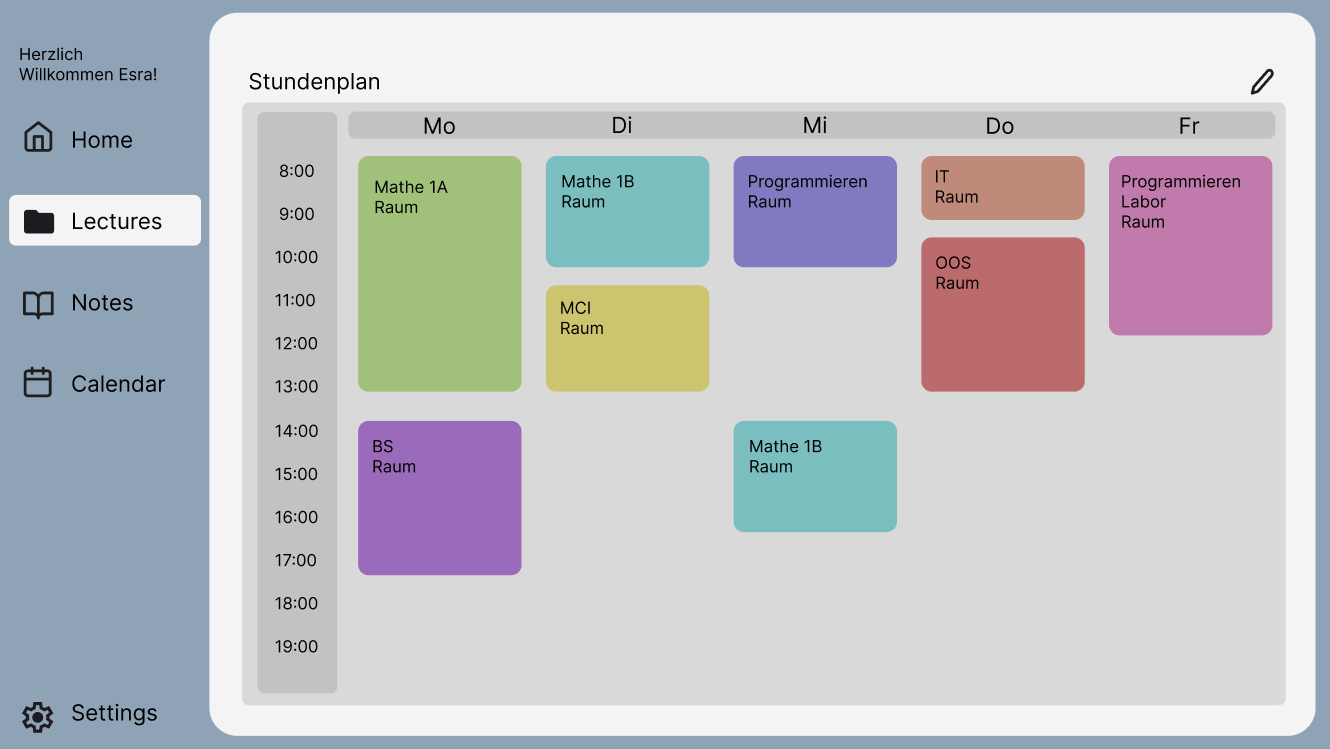
\includegraphics[width=1\textwidth]{./images/lecturepage.png}
  \caption{Stundenplan}
  \label{fig:lectures}
\end{figure}
 Die Abbildung \ref{fig:notes} zeigt das Notizmodul, in dem Studierende ihre Lernmaterialien organisieren können.
\begin{figure}[H]
  \centering
  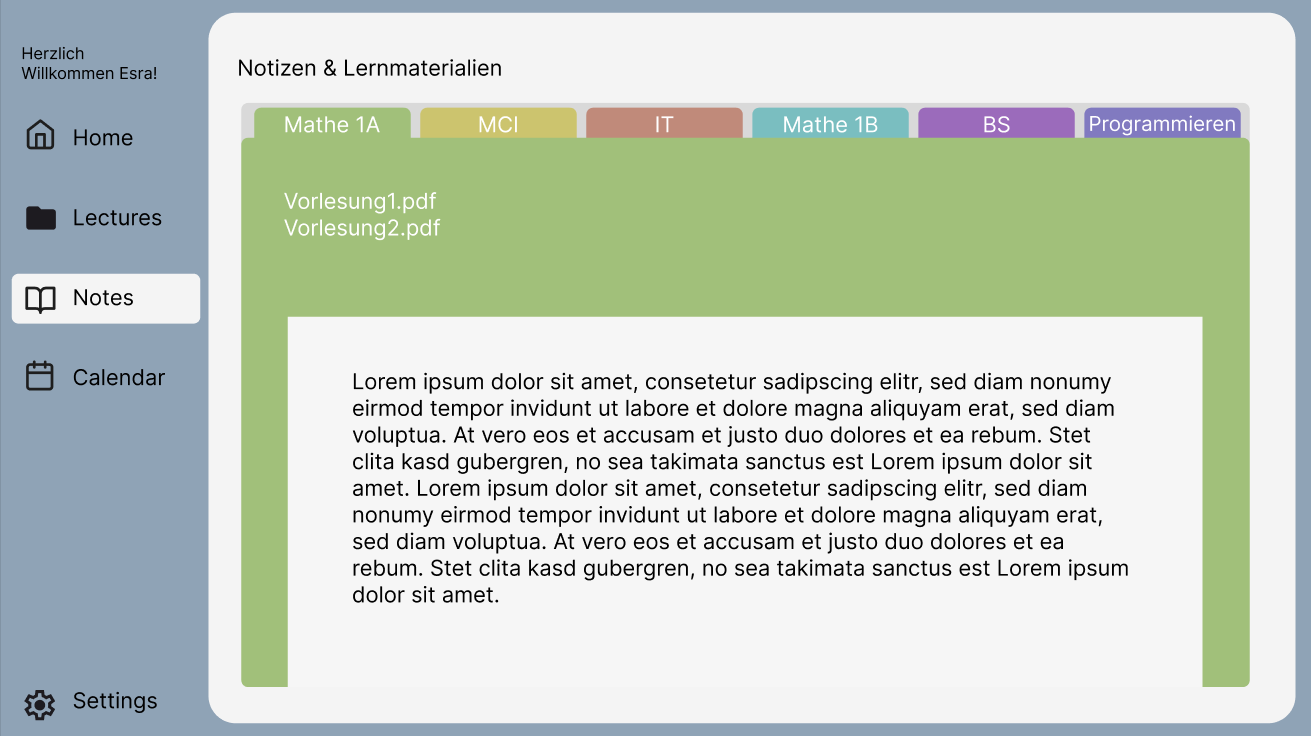
\includegraphics[width=1\textwidth]{./images/notespage.png}
  \caption{Notizen und Lernmaterialien}
  \label{fig:notes}
\end{figure}
Abbildung \ref{fig:calendar-1} und \ref{fig:calendar-2} zeigen den Kalender, in dem Prüfungstermine und Fristen eingetragen werden können. Nutzer:innen können neue Einträge hinzufügen und bestehende verwalten.
\begin{figure}[H]
  \centering
  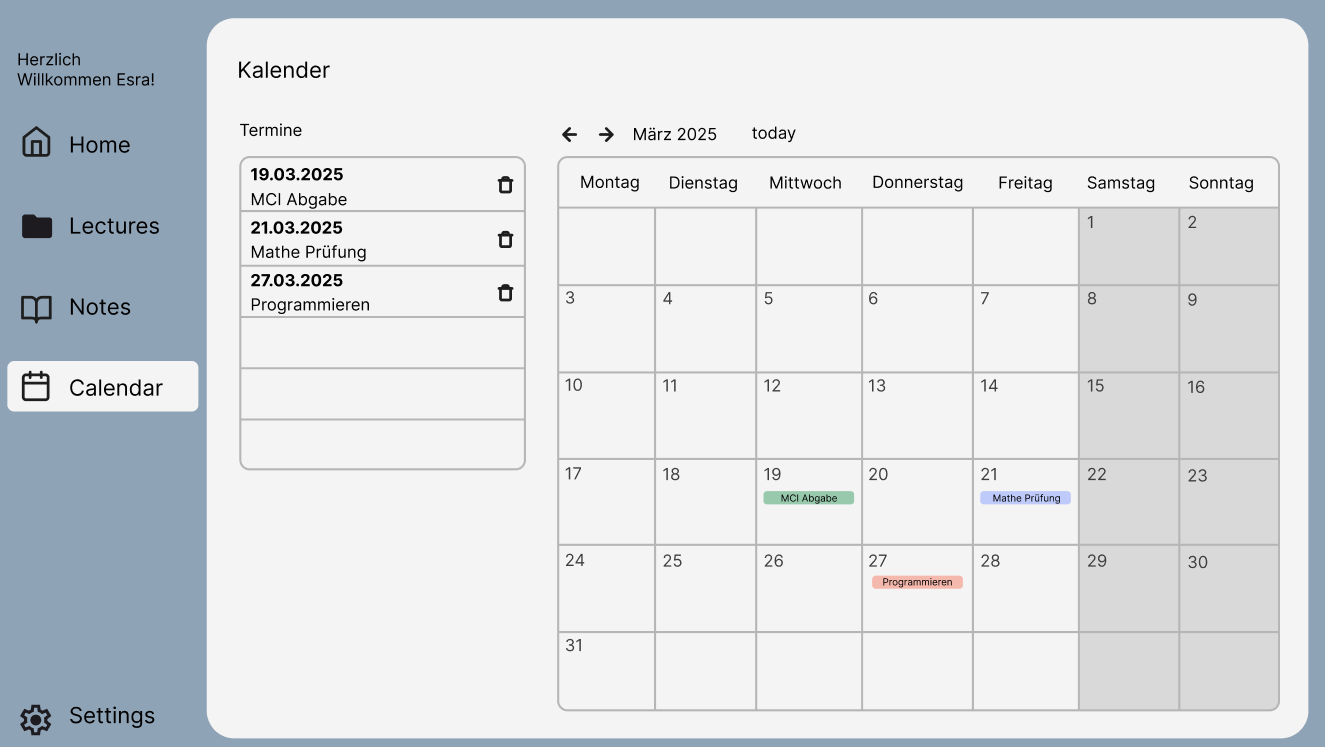
\includegraphics[width=1\textwidth]{./images/calendarpage-1.png}
  \caption{Kalender}
  \label{fig:calendar-1}
\end{figure}

\begin{figure}[H]
  \centering
  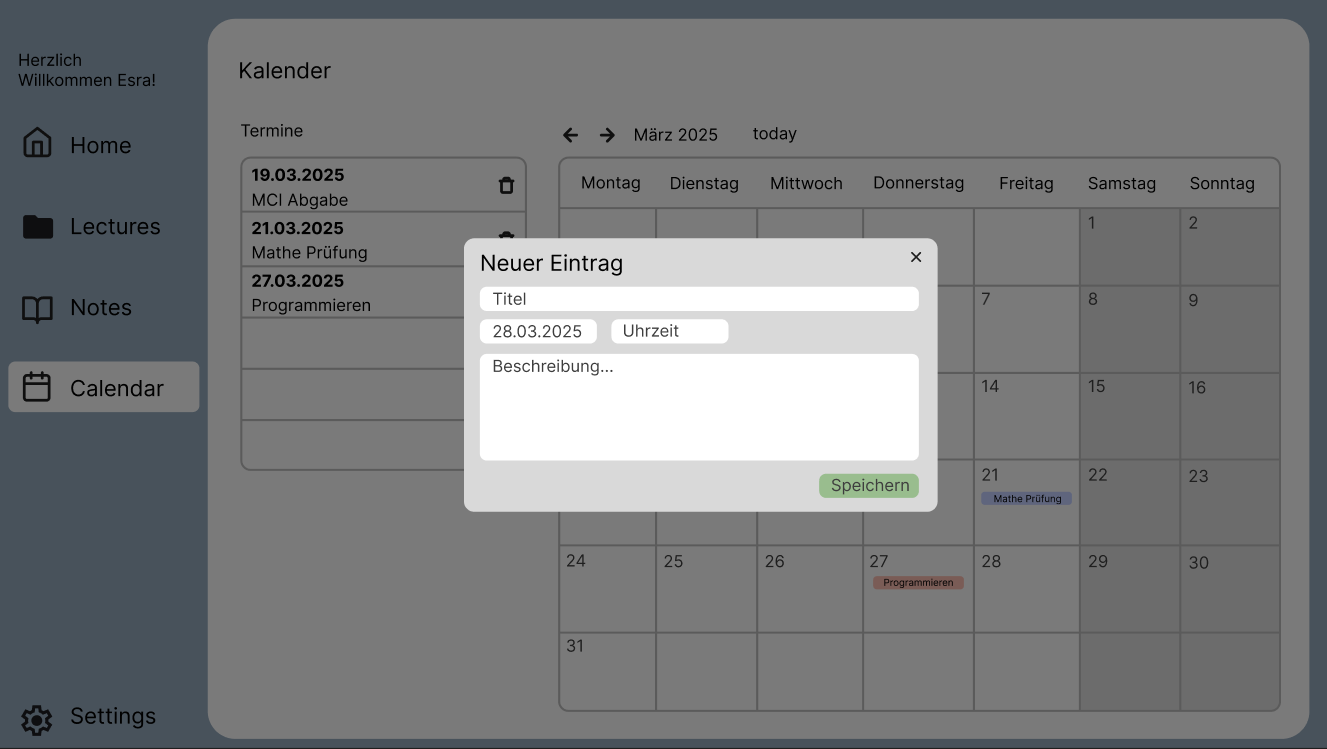
\includegraphics[width=1\textwidth]{./images/calendarpage-2.png}
  \caption{Neuen Eintrag in den Kalender einfügen}
  \label{fig:calendar-2}
\end{figure}